\documentclass[oneside,a4paper,11pt,explicit]{book}
\usepackage[utf8]{inputenc}
\usepackage{kultem}

\usepackage[hidelinks]{hyperref}
\usepackage{lipsum}

\title{Simple Example}
\subtitle{Of the kultem style}
\date{\today}
\author{Henri De Plaen}
\date{February 2021}
\professor{Prof. Nice Teacher}

\begin{document}

\maketitle

\chapter{Introduction}
\kulbox{{\bf Note:} This is a nice box where you can put a lot of information concerning the following chapter. How much pages are required for an assignment for example, or an important change of notation.}
\lipsum[1]

\section{Some questions}
\lipsum[2] \\

As an example, we will consider the equation of the Duffing oscillator
\begin{equation}
\ddot{x}+k\dot{x}+x^3=B\cos t,
\end{equation}
with $k=0.1$ and $B=11$ and answer the following questions

\begin{questions}
\question Can you show that the model exhibits a chaotic regime?
\begin{tasks}
\task By performing a qualitative analysis of a simulation?
\task By computing the Lyapunov exponents of the system?
\end{tasks}
\question What is the dimension of the system?
\question Simulate the model for another choice of parameters. What do you observe?
\end{questions}

\section{Some figures}
\lipsum[3] This can be seen at figure~\ref{fig:example}.

\begin{figure}[h]
    \centering
    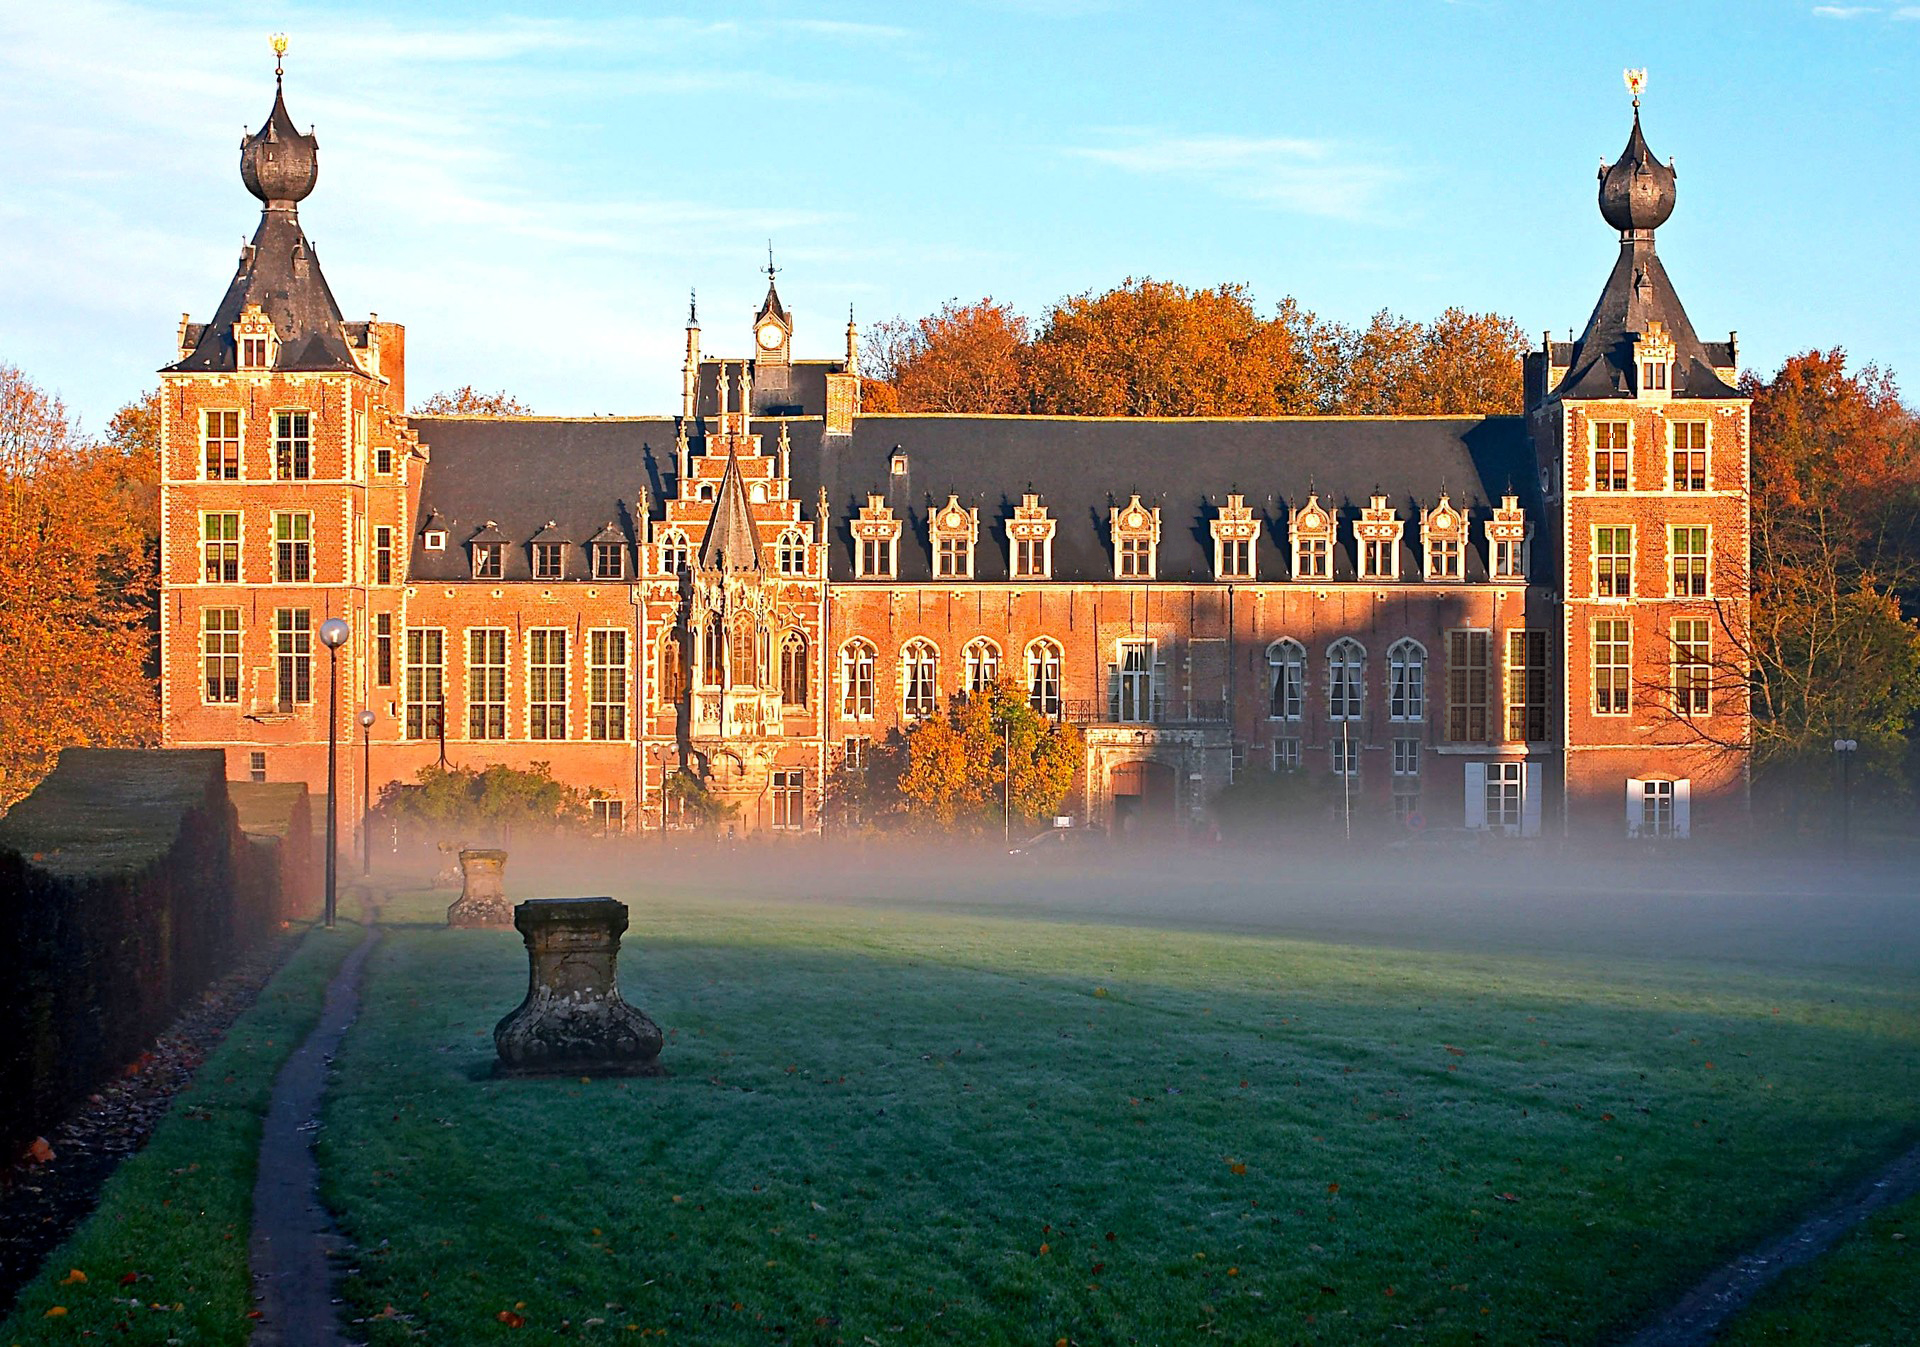
\includegraphics[width=\textwidth]{./arenberg.jpg}
    \caption{The castle of Arenberg in Heverlee, with windows corrected.}
    \label{fig:example}
\end{figure}


\end{document}
